\documentclass{article}
\usepackage{graphicx}
\usepackage[margin=1.5cm]{geometry}
\usepackage{amsmath}

\begin{document}

\title{Lab Activity: Smashing Things Together (Momentum)}
\author{Prof. Jordan C. Hanson}

\maketitle

\section{Introduction}
This lab activity demonstrates momentum conservation through the use of carts that repel each other via magnets, and also simply collide.  Figure \ref{fig:carts} demonstrates the general setup.
\begin{figure}[ht]
\centering
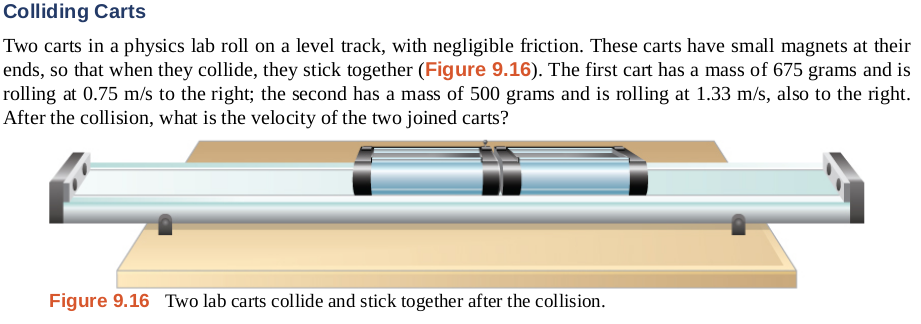
\includegraphics[width=0.6\textwidth]{figures/carts.png}
\caption{\label{fig:carts} Carts that collide with different interaction properties.}
When momentum is conserved between two objects labeled 1 and 2, with $i$ and $f$ referring to the initial and final states,
\begin{equation}
p_{1i} + p_{2i} = p_{1f} + p_{2f}
\end{equation}
\end{figure}

\section{Predicting Velocity}

Set two carts with equal mass on the frictionless track and knock them together at \textbf{low speed}.  (a) Use the motion detector to measure the velocity of one cart going toward and away from the interaction, with the magnetic sides of the carts facing each other and repelling each other.  Record the mass below in meters per second.  (b) Now alter the mass of one of the carts by placing weights on it, and record the ingoing and outgoing velocity.  \\ \vspace{1.5cm}

Explain your observations using momentum conservation, and assuming that kinetic energy is also conserved.  (a) Write an equation for momentum conservation governing the two carts, and assume they have the same mass.  Similarly, write an equation for kinetic energy conservation, and assume the two carts have the same mass.  Calculate what the velocity of the cart \textit{should be} by combining kinetic energy and momentum conservation, and compare to your measurements.  (b) Repeat for the data collected when the carts had different masses.

\end{document}